\chapter{Audioausgabe}
\label{Audioausgabe}
% ================ Einstellungen =======================
\thispagestyle{fancy} \rhead{\slshape Audioausgabe} 
% ======================================================
In diesem Kapitel werden die technischen Grundlagen welche sich auf das verwendete Audio-Modul beziehen, das Konzept sowie die Funktion der Audioausgabe beschrieben. Zudem wird die Validierung erläutert.
\section{Technische Grundlagen}
Für den Prototyp des Dojo’s wurde unter anderem ein WTV020 Chip verwendet. Das WTV020 Modul wird in diesem Kapitel beschrieben, da diese Informationen für die nachfolgenden Kapitel benötigt werden.\\
Das WTV020 Modul ist ein Soundmodul welches es ermöglicht Audiodateien auf einem Aktor abzuspielen. Auf einer maximal 1GB grossen $\mu$SD-Karte können bis zu 512 Audiodateien abgespeichert werden. Die Audiodateien auf der $\mu$SD-Karte müssen jedoch dem .wav oder.ad4 Format entsprechen. Die Dateien müssen gemäss Vorgabe: 0000; 0001; 0002; … nummeriert werden.\\
Der WTV020 Chip kann in zwei verschiedenen Modes betrieben werden, dem MP3 Mode und dem Two Line Serial Mode. Im MP3 Mode können direkt 6 Pins angesteuert werden. Durch die sechs Pins können folgende Funktionen umgesetzt werden: Reset, $\pm$Volume , next, previous und play, pause. 
Für das Dojo wird jedoch der two line serial mode genützt. Dieser kann das Modul mit nur 3 Pins betreiben. Der Mikrocontroller muss an den Clock-, den Data- und den Busy-Pin angeschlossen werden. Im two line serial mode können die Audiodateien welche sich auf der $\mu$SD-Karte befinden abgespielt werden. Er ermöglicht zudem, ähnlich wie im MP3 Mode ein Lied zu pausieren und neu zu starten, sowie eine Lautstärkenregulation.
\section{Konzept}
Das Konzept der Audioausgabe ist wie folgt aufgebaut:
\begin{figure}[h]
	\centering
	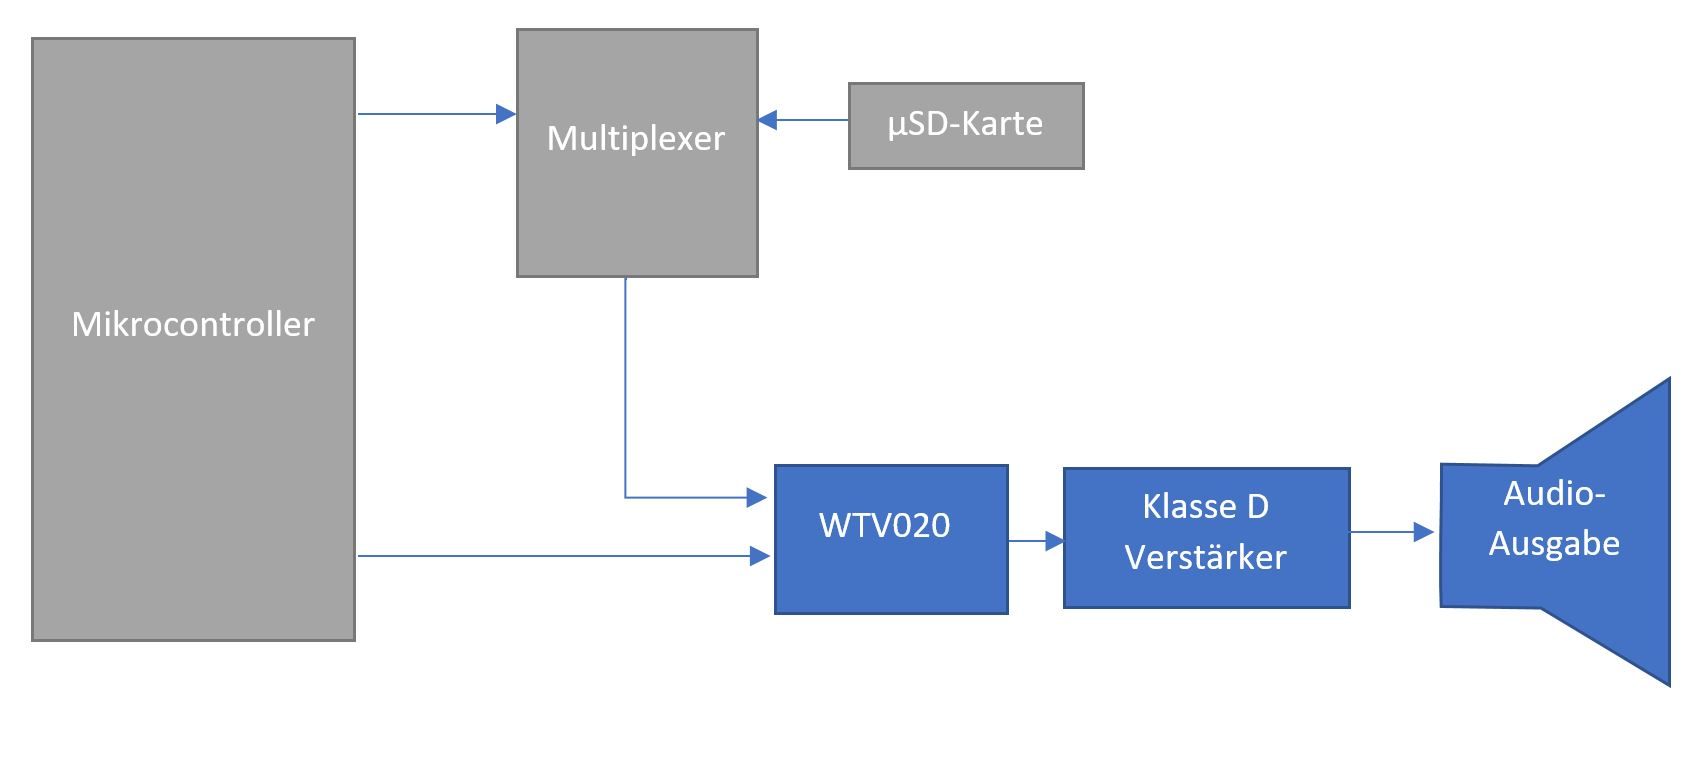
\includegraphics[width=15cm]{Bilder/Audio-Konzept.jpg}
	\caption{Audio Konzept}
	\label{Audio-Konzept}
\end{figure}
Die auf einer $\mu$SD-Karte abgespeicherten Audiodateien werden über einen Multiplexer, welcher vom Mikrocontroller gesteuert wird, an einen WTV020 Chip übertragen. Dieser wird in einem Serial Mode [Kapitel WTv020] betrieben und kann ebenfalls vom Mikrocontroller angesteuert werden. Der Audiochip entschlüsselt die Daten und gibt diese an einen Klasse D Verstärker weiter. Dieser wird benötigt um eine gut hörbare Lautstärke zu erreichen. Das Audiosignal wird schliesslich an einem Bone Conductor ausgegeben. 
Nachfolgend wird die Anordnung auf dem Print der einzelnen Komponenten dargelegt. 
\section{Hardware}
Wie im Konzept beschrieben, muss man, um Daten von der $\mu$SD-Karte auszulesen zuerst den Multiplexer ansteuern. Dies geschieht über den Mikrocontroller. Im ungesteuerten Zustand ist der MUX auf den VUB300 geschaltet. Sobald der MUX entsprechend angesteuert wird schalten die benötigten Kontakte. Der WTV020SD-20S Chip kann nun auf die $\mu$SD-Karte zugreifen. Über vier Pins werden die Audiofiles ausgelesen und weitergegeben. Das Audiosignal wird auf den Klasse-D Verstärker gegeben. Dieser ist wie folgt aufgebaut.
\begin{figure}[h]
	\centering
	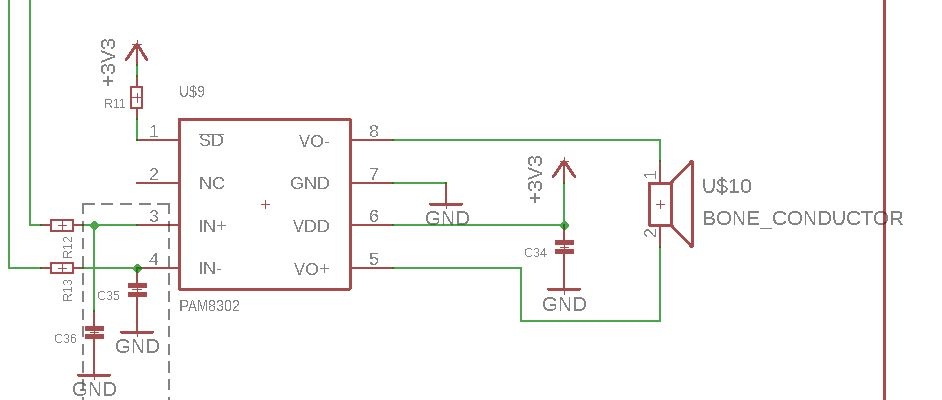
\includegraphics[width=15cm]{Bilder/Klasse-D.jpg}
	\caption{Klasse D Verstärker}
	\label{Klasse-D}
\end{figure}
Um ein Rauschen an der Speisung zu vermeiden wird ein ein$\mu$ Farad grosser Kondensator benötigt. In diesem Projekt wurde eine konstante Verstärkung mit dem Faktor ca.15 verwendet, da die Lautstärken Regelung über den WTV020-Chip geregelt werden soll. Dieser Faktor entsteht aus dem Verhältnis der Widerstände. Um das Rauschen der Eingänge sowie zu hohe Frequenzen zu filtern wurden zuerst wie die Abbildung \ref{Klasse-D} zeigt, Kapazitäten eingeplant. Auf dem Prototyp wurden aufgrund von Tests welche in der Validierung aufgeführt werden, die Kapazitäten weggelassen.\\ Wie erwähnt wird die Lautstärkenregelung über den WTV020-Chip geregelt. Dies ist jedoch im serial mode fehleranfällig. Aufgrund dessen wurde für die Tests ein 50 Ohm grosser Widerstand vor den Bone Conductor geschaltet da bei grossen Strömen dieser eine zu kleine Innenimpedanz aufweist.\\ Wie erwähnt wird die Lautstärkenregelung über den WTV020-Chip geregelt. Dies ist jedoch im serial mode fehleranfällig. Aufgrund dessen wurde für die Tests ein 50 Ohm grosser Widerstand vor den Bone Conductor geschaltet da bei grossen Strömen dieser eine zu kleine Innenimpedanz aufweist. Die Audioausgabe erfolgt wie beschrieben über einen Bone Conductor. Der Bone Conductor besteht aus einem kleinen Metallstab welcher mit einer Kupfer Spule umwickelt ist. Sobald ein pulsförmiger Strom durch die Spule fliest, dehnt sich ein Magnetfeld aus welches ein zusammenziehen auslöst. Der Bone Conductor ermöglicht es durch die Vibrationen das eine Audio Datei über den Schädelknochen abgespielt wird und so nur für eine Person hörbar ist, diese jedoch immer noch die Umgebungsgeräusche war nimmt.

\section{Firmware}

\section{Validierung}